\documentclass[11pt]{amsart}

\usepackage[T1]{fontenc}
\usepackage{lmodern}
\usepackage{amssymb,amsmath}
\usepackage{booktabs,array}
\usepackage{graphicx}
\usepackage[dvipsnames]{xcolor}
\usepackage[margin=1.15in]{geometry}
\usepackage[colorlinks=true,linkcolor=blue!50!black,citecolor=blue!50!black,urlcolor=blue!50!black]{hyperref}

\newtheorem{theorem}{Theorem}[section]
\newtheorem{proposition}[theorem]{Proposition}
\newtheorem{lemma}[theorem]{Lemma}
\newtheorem{corollary}[theorem]{Corollary}
\theoremstyle{definition}
\newtheorem{definition}[theorem]{Definition}
\newtheorem{innerconj}{Conjecture}
\newenvironment{conjecture}[1]{\renewcommand{\theinnerconj}{#1}\innerconj}{\endinnerconj}
\theoremstyle{remark}
\newtheorem{remark}[theorem]{Remark}

\numberwithin{equation}{section}

\newcommand{\sco}{\operatorname{sc}}
\hypersetup{pdftitle={A short proof that link-irregular tournaments exist for every order at least six},pdfauthor={Deep Bhattacharjee}}
\providecommand{\doi}[1]{\url{https://doi.org/#1}}

\begin{document}

\title[Link-irregular tournaments]{A short proof that link-irregular tournaments\\ exist for every order at least six}

\author{Deep Bhattacharjee}
\address{Formerly, Electro-Gravitational Space Propulsion Laboratory (EGSPL),\newline Bhubaneswar, Odisha 751030, India}
\email{d.bhattacharjee@erl-forschung.de}
\email{itsdeep@live.com}
\urladdr{https://orcid.org/0000-0003-0466-750X}
\thanks{Corresponding author: \href{mailto:d.bhattacharjee@erl-forschung.de}{d.bhattacharjee@erl-forschung.de}; ORCID \href{https://orcid.org/0000-0003-0466-750X}{\mbox{0000-0003-0466-750X}}}

\subjclass[2020]{Primary 05C20; Secondary 05C60}
\keywords{tournament, link-irregular digraph, vertex-deleted subtournament, score sequence}

\begin{abstract}
A digraph is link-irregular if no two of its vertices have isomorphic links. Bastien and Khormali conjectured that a link-irregular tournament on $n$ vertices exists if and only if $n\ge6$, and Chau proved it by substitution into a transitive tournament. We give a short different proof, by a construction that adds two vertices at a time.
\end{abstract}

\maketitle

\section{Introduction}

The link $L_D(v)$ of a vertex $v$ in a digraph $D$ is the subdigraph induced by the in- and out-neighbours of $v$, and $D$ is \emph{link-irregular} if $L_D(u)\not\cong L_D(v)$ for all distinct vertices $u,v$. Links of vertices in graphs were introduced by Ali, Chartrand and Zhang~\cite{ACZ}, and Bastien and Khormali~\cite{BK} carried the notion over to digraphs. In a tournament every other vertex is a neighbour of $v$, so the link of $v$ is the subtournament $T-v$. A tournament is therefore link-irregular exactly when its $n$ vertex-deleted subtournaments are pairwise non-isomorphic.

Bastien and Khormali showed that there is no link-irregular tournament on $n\le5$ vertices (for $n=5$ there are only four tournaments on four vertices, up to isomorphism, to serve as links), gave link-irregular tournaments on $6$, $7$ and $8$ vertices, and found examples by computer search for every $n\le100$. Their construction adds one dominating vertex at a time and stops working at $9$ vertices. They made the following conjecture (\cite[Conjecture~6]{BK}; Conjecture~3.7 in the journal version~\cite{BKj}).

\begin{conjecture}{1}\label{conj}
A link-irregular tournament on $n$ vertices exists if and only if $n\ge6$.
\end{conjecture}

Here $n\ge2$; the tournament with one vertex is link-irregular for want of a second vertex.

Chau~\cite{Chau} proved Conjecture~\ref{conj}. Call a tournament $2$-strong if it is strongly connected and stays so after any one vertex is deleted. Chau showed that substituting link-irregular $2$-strong tournaments into a transitive tournament gives a link-irregular tournament, and he found such tournaments of every order from $8$ to $15$ by computer search; together with the examples of Bastien and Khormali this covers every $n\ge6$. Harte formalised Chau's proof in Lean~\cite{HarteLean} and showed that $7$ is the least order of a link-irregular $2$-strong tournament~\cite{Harte}.

We give a second proof. Its only finite input is a pair of tournaments on six and seven vertices whose links can be told apart by hand.

\begin{theorem}\label{thm:main}
For every $n\ge6$ there is a link-irregular tournament on $n$ vertices that has neither a source nor a sink.
\end{theorem}

The proof is an induction from $n$ to $n+2$ (Lemma~\ref{lem:step}), started at $n=6$ and $n=7$ (Section~\ref{sec:base}). The new pair of vertices is a source and a sink of the old tournament joined by one reversed arc; this pair can be recognised inside every link, which is what makes the step work.

We write $u\to v$ when the arc between $u$ and $v$ points from $u$ to $v$, and $\sco_T(v)$ for the score (out-degree) of $v$ in a tournament $T$. A source of $T$ is a vertex of score $|T|-1$ and a sink is a vertex of score $0$. Isomorphisms of tournaments preserve scores.

\section{The step from $n$ to $n+2$}

Let $T$ be a tournament on a vertex set $V$ with $|V|=n$. Let $T^+$ be the tournament on $V\cup\{s,t\}$ that contains $T$ and has the arcs
\[
s\to v\ \text{ and }\ v\to t\quad (v\in V),\qquad t\to s
\]
(Figure~\ref{fig:step}). In $T^+$ we have $\sco(s)=n$, $\sco(t)=1$ and $\sco(v)=\sco_T(v)+1$ for $v\in V$.

\begin{figure}[ht]
\centering
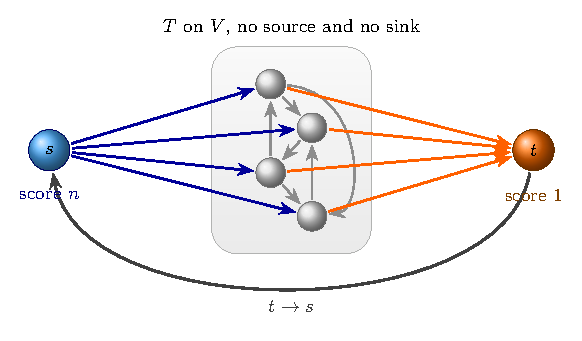
\includegraphics[width=0.8\textwidth]{figures/step}
\caption{The tournament $T^+$: $s$ beats every vertex of $T$, every vertex of $T$ beats $t$, and $t$ beats $s$.}
\label{fig:step}
\end{figure}

\begin{lemma}\label{lem:step}
Let $n\ge3$ and let $T$ be a link-irregular tournament on $n$ vertices with neither a source nor a sink. Then $T^+$ is a link-irregular tournament on $n+2$ vertices with neither a source nor a sink.
\end{lemma}

\begin{proof}
Since $1\le\sco_T(v)\le n-2$ for $v\in V$, the scores in $T^+$ lie between $1$ and $n$, while $T^+$ has $n+2$ vertices; so $T^+$ has no source and no sink. We compare the links $T^+-x$ for $x\in V\cup\{s,t\}$, each of which has $n+1$ vertices, so that a source in it has score $n$.

\emph{The link of $s$.} In $T^+-s$ the vertex $t$ has score $0$, so $T^+-s$ has a sink. Every $v\in V$ has score $\sco_T(v)+1\le n-1$ there, so $T^+-s$ has no source.

\emph{The link of $t$.} In $T^+-t$ the vertex $s$ has score $n$, so $T^+-t$ has a source. Every $v\in V$ has score $\sco_T(v)\ge1$ there, so $T^+-t$ has no sink.

\emph{The link of $v\in V$.} In $T^+-v$ the vertex $s$ has score $n-1$, the vertex $t$ has score $1$, and $u\in V\setminus\{v\}$ has score $\sco_{T-v}(u)+1$, which lies between $1$ and $n-1$. So $T^+-v$ has neither a source nor a sink.

Hence the link of $s$, the link of $t$ and the links of vertices of $V$ fall into three classes that no isomorphism can mix: the first has a sink but no source, the second a source but no sink, the third neither.

It remains to show $T^+-v\not\cong T^+-w$ for distinct $v,w\in V$. Call a vertex $y$ of $T^+-v$ \emph{marked} if $\sco(y)=1$ and the unique out-neighbour of $y$ has score $n-1$. The vertex $t$ is marked, its out-neighbour being $s$. Any other vertex of score $1$ in $T^+-v$ is some $u\in V\setminus\{v\}$ with $\sco_{T-v}(u)=0$; its only out-neighbour is $t$, whose score is $1\ne n-1$ because $n\ge3$. So $t$ is the only marked vertex of $T^+-v$, and $s$ is its out-neighbour. The same holds in $T^+-w$. An isomorphism $\varphi\colon T^+-v\to T^+-w$ preserves scores and arcs, hence maps the marked vertex to the marked vertex, so $\varphi(t)=t$ and then $\varphi(s)=s$. Its restriction is an isomorphism from $T-v$ onto $T-w$, which is impossible because $T$ is link-irregular.
\end{proof}

\section{Two starting tournaments}\label{sec:base}

Let $T_6$ be the tournament on $\{1,\dots,6\}$ with the arcs
\[
1\to2,3,4,5;\quad 2\to3,4,5,6;\quad 3\to4,6;\quad 4\to5,6;\quad 5\to3;\quad 6\to1,5,
\]
where $i\to j,k$ means $i\to j$ and $i\to k$; the pairs not listed are oriented the other way. Its scores are $4,4,2,2,1,2$, so it has no source and no sink. Let $T_7$ be the tournament on $\{1,\dots,7\}$ with the arcs
\[
1\to2,3,4,5,6;\quad 2\to3,4,5,6,7;\quad 3\to4,5,7;\quad 4\to5,6,7;\quad 5\to6;\quad 6\to3;\quad 7\to1,5,6,
\]
with scores $5,5,3,3,1,1,3$; it has no source and no sink either.

\begin{lemma}\label{lem:base}
$T_6$ and $T_7$ are link-irregular.
\end{lemma}

\begin{proof}
Table~\ref{tab:base} lists the score sequence of every vertex-deleted subtournament; each entry is obtained by deleting one vertex and recounting out-degrees. For $T_7$ the seven sequences are distinct, so the seven links are pairwise non-isomorphic. For $T_6$ the sequences are distinct except for $T_6-4$ and $T_6-5$, which both have score sequence $(1,1,2,3,3)$. In $T_6-4$ the unique vertex of score $2$ is $6$, and it beats vertex $1$, which has score $3$. In $T_6-5$ the unique vertex of score $2$ is $3$, and it beats only the vertices $4$ and $6$, both of score $1$. An isomorphism would carry the vertex of score $2$ to the vertex of score $2$ and preserve the scores of its out-neighbours, so $T_6-4\not\cong T_6-5$.
\end{proof}

\begin{table}[ht]
\centering
\caption{Score sequences (in increasing order) of the vertex-deleted subtournaments of $T_6$ and $T_7$.}
\label{tab:base}
\begin{tabular}{c c @{\qquad\qquad} c c}
\toprule
$v$ & score sequence of $T_6-v$ & $v$ & score sequence of $T_7-v$\\
\midrule
1 & $(1,1,2,2,4)$ & 1 & $(1,1,2,3,3,5)$\\
2 & $(1,2,2,2,3)$ & 2 & $(1,1,3,3,3,4)$\\
3 & $(0,2,2,3,3)$ & 3 & $(0,1,3,3,4,4)$\\
4 & $(1,1,2,3,3)$ & 4 & $(1,1,2,3,4,4)$\\
5 & $(1,1,2,3,3)$ & 5 & $(1,2,2,2,4,4)$\\
6 & $(1,1,1,3,4)$ & 6 & $(0,2,2,3,4,4)$\\
  &                & 7 & $(1,1,2,2,4,5)$\\
\bottomrule
\end{tabular}
\end{table}

\begin{proof}[Proof of Theorem~\ref{thm:main}]
Put $T_{n+2}=T_n^+$ for $n\ge6$. Starting from $T_6$ and $T_7$, Lemmas~\ref{lem:base} and~\ref{lem:step} show by induction on $n$ that $T_n$ is a link-irregular tournament on $n$ vertices without a source or a sink, for every $n\ge6$. For $2\le n\le5$ no link-irregular tournament exists, as Bastien and Khormali observed~\cite[Observation~7]{BK}: the $n$ links are tournaments on $n-1$ vertices, and up to isomorphism there are only $1,1,2,4$ tournaments on $1,2,3,4$ vertices, fewer than $n$ in each case.
\end{proof}

\begin{remark}
The construction is explicit: $T_n$ is obtained from $T_6$ or $T_7$ by adding the pairs $(s_1,t_1),(s_2,t_2),\dots$ in turn, where $s_i$ beats all earlier vertices except $t_i$, all earlier vertices beat $t_i$, and $t_i\to s_i$. The proof of the step uses the absence of a source and a sink in $T$, and this is exactly what it hands on to $T^+$. Going through the $2^{15}$ tournaments on six vertices shows that $T_6$ is one of exactly four link-irregular tournaments on six vertices up to isomorphism, and that none of the four has a source or a sink. On seven vertices there are $139$, eight of which have a source or a sink. Since an automorphism of a tournament maps each link onto an isomorphic link, a link-irregular tournament has no automorphism other than the identity.
\end{remark}

\begin{remark}
Every link-irregular tournament on $n\ge 6$ vertices whose links have pairwise different score sequences gives such a tournament on $n+2$ vertices with the same property, because the score sequence of $T^+-v$ is that of $T-v$ with every entry raised by one and the entries $1$ and $n-1$ added. Starting from $T_7$, this gives link-irregular tournaments of every odd order whose links are already told apart by their score sequences.
\end{remark}

\subsection*{Use of generative AI} The author used Claude (Anthropic) for literature search, computation and drafting; the author checked the mathematics and takes full responsibility for the content.

\begin{thebibliography}{9}

\bibitem{ACZ}
A.~Ali, G.~Chartrand and P.~Zhang, \emph{On link-irregular graphs}, Discuss. Math. Graph Theory \textbf{45} (2025). \doi{10.7151/dmgt.2521}

\bibitem{BK}
A.~Bastien and O.~Khormali, \emph{On link-irregular digraphs}, preprint, 2025. \href{https://arxiv.org/abs/2512.20494}{arXiv:2512.20494}

\bibitem{BKj}
A.~Bastien and O.~Khormali, \emph{On link-irregular digraphs}, J. Combin. Math. Combin. Comput. \textbf{130} (2026), 227--240. \doi{10.61091/jcmcc130-15}

\bibitem{Chau}
C.~H. Chau, \emph{A proof of the Bastien--Khormali conjecture on link-irregular tournaments}, preprint, 2026. \doi{10.5281/zenodo.22150037}

\bibitem{Harte}
S.~Harte, \emph{The minimal base order for the join construction on link-irregular tournaments}, preprint, 2026. \doi{10.5281/zenodo.22232944}

\bibitem{HarteLean}
S.~Harte, \emph{A Lean~4 formalisation of the Bastien--Khormali conjecture and the minimal base order for Chau's join construction}, software, 2026. \doi{10.5281/zenodo.22232432}

\end{thebibliography}

\end{document}
